%%%%%%%% VERISIEVE TECHNICAL NOTE (MLSYS TWO-COLUMN LAYOUT KIT) %%%%%%%%%%
% Compile: pdflatex mlsys2027-verisieve && bibtex mlsys2027-verisieve && pdflatex ... x2
%%%%%%%%%%%%%%%%%%%%%%%%%%%%%%%%%%%%%%%%%%%%%%%%%%%%%%%%%%%%%%%%%%%%%%%%
\documentclass{article}

\usepackage[T1]{fontenc}
\usepackage{microtype}
\usepackage{graphicx}
\usepackage{booktabs}
\usepackage{amsmath}
\usepackage{amssymb}
\usepackage{hyperref}

\newcommand{\theHalgorithm}{\arabic{algorithm}}

\usepackage[accepted]{mlsys2025}

% Override mlsys2025 footer/metadata so this compiles cleanly as a Technical Note
\makeatletter
\renewcommand{\mlsys@appearing}{VeriSieve Technical Note --- RTIO / VeriSieve / MLE Architecture \& Empirical Audit (Nov 2026). Copyright 2026 Gege Ardiyansyah.}
\renewcommand{\Notice@String}{\mlsys@appearing}
\makeatother

\hypersetup{
  pdftitle={VeriSieve: Deterministic Zero-Egress Document Curation and Conformal Gatekeeping},
  pdfauthor={Gege Ardiyansyah},
  pdfsubject={Technical Note}
}

\mlsystitlerunning{VeriSieve Technical Note: Zero-Egress Curation, Conformal Triage, and Substrate Benchmarks}

\begin{document}

\twocolumn[
\mlsystitle{VeriSieve Technical Note: Deterministic Document Curation, Customer-Label Conformal Gatekeeping, and Substrate Benchmarks}

\begin{mlsysauthorlist}
\mlsysauthor{Gege Ardiyansyah}{ind}
\end{mlsysauthorlist}
\mlsysaffiliation{ind}{Maincode / Independent Research, Melbourne, Australia}
\mlsyscorrespondingauthor{Gege Ardiyansyah}{https://github.com/gegearsyah/verisieve}

\mlsystitlerunning{VeriSieve Technical Note: Zero-Egress Curation, Conformal Triage, and Substrate Benchmarks}
\mlsyskeywords{WebAssembly, conformal prediction, Learn-Then-Test, PII de-identification, document curation, systems measurement}

\vskip 0.3in

\begin{abstract}
Client-side AI post-training requires deterministic data preparation and strict quality gating without egressing raw records to third-party endpoints. We report the architecture and same-session empirical evaluation of \textbf{VeriSieve}, the portable curation and conformal gatekeeper engine behind the \textbf{RTIO} interactive sandbox (\url{https://www.rtio.io/sandbox}), paired with \textbf{MLE's \texttt{mle\_dl\_*} WebAssembly kernels} (\texttt{verisieve\_dl.wasm}) for BitNet/VeRA adapter training and 64-dimensional needle retrieval. Rather than projected estimates, every measurement executes directly across $1,207$ benchmark documents: ICDAR-2019 FUNSD ($199$ forms, $30,595$ word boxes), PubMedQA ($500$ clinical abstracts), PubMed Central full-text clinical PDFs ($8$ papers, $55,099$ words), and \texttt{ai4privacy-200k} ($500$ synthetic span-annotated records). We measure: (1) deterministic text ingestion (\texttt{.docx} OOXML XML extraction in $0.41$\,ms, HTML boilerplate stripping of $53.7\%$ in $0.83$\,ms, SHA-256 + 3-gram Jaccard deduplication, and scoped \texttt{/ToUnicode} CMap + negative-kerning \texttt{TJ} reconstruction extracting $8/8$ PMC PDFs---$8,134$ readable lines---in $111.86$\,ms without image OCR), alongside $97.38\%$ FUNSD geometric bounding-box survival under $512{\times}512$ 2D overlapping tiling vs.\ $20.53\%$ untiled; (2) PII rule boundaries showing $97.1\%$ recall on contact/card/IPv4 spans, an honest $49.6\%$ regex ceiling on bare names ($42.1\%$ across all $26$ structured tags), and a pre-committed $334$-word lexicon cutting blind PubMedQA Title-Case false positives $2.72\times$ ($5.46 \to 2.01$ hits/1k words); (3) single-scorer Learn-Then-Test (LTT) calibration ($\delta=0.05$) achieving monotonic held-out risk control ($14.8\% \to 0.0\%$ conditional FPR, $9.67\% \to 0.0\%$ joint risk), explicit fail-closed calibration on $n_{\text{cal,unsafe}}=196 < 299$ at $\alpha=0.01$ ($43.67\%$ abstain), and $100$-label customer multi-axis triage (\texttt{safe} $\land$ \texttt{useful} $\land$ \texttt{topic}) with $90.7\%$ gold-yield retention and $0.0\%$ unsafe leak; and (4) 7-trial interleaved OS process-spawn timings across C99 ($8.35$\,ms spawn, $6.07$\,MB RSS, $0.38$\,ms hot), Node+WASM ($54.63$\,ms spawn / $1.35$\,ms warm WASM init, $51.21$\,MB RSS, $0.48$\,ms hot), Python+NumPy ($232.51$\,ms spawn, $31.44$\,MB RSS, winning warm BLAS at $0.085$\,ms), and Python+PyTorch+DuckDB ($7,237.8$\,ms spawn, $432.6$\,MB RSS), alongside held-out ablation reducing 520-dim gate BCE loss by $27.7\%$ ($0.3133 \to 0.2266$, $93.3\%$ accuracy) and WASM VeRA BCE loss from $0.6869 \to 0.5529$.
\end{abstract}
]

\printAffiliationsAndNotice{}

\section{Introduction \& Stack Positioning}
\label{sec:intro}

Domain-specific post-training and retrieval pipelines ingest heterogeneous institutional records---research PDFs, Word documents, scraped web articles, and scanned archival forms \citep{soldaini2024dolma,penedo2024fineweb}. In clinical, legal, and proprietary enterprise workflows, raw records cannot be transmitted to external cloud APIs for PII redaction or LLM-based quality filtering \citep{ai4privacy2023,presidio2021}. Everything must run deterministically inside an auditable client or edge sandbox.

To separate interface, portable curation logic, and compiled numerical kernels, our stack follows a strict three-tier boundary:
\begin{enumerate}
    \item \textbf{RTIO} (\url{https://www.rtio.io/sandbox}) serves as the interactive web interface where users load URLs, documents, or shard presets, inspect redactions and conformal abstentions live, label chunks, and trigger local training runs.
    \item \textbf{VeriSieve} acts as the portable deterministic engine behind RTIO, executing identical parsing, deduplication, PII disambiguation, 520-dimensional feature extraction, and LTT binomial gatekeeping across the browser, Node.js CLI, the Model Context Protocol (MCP), and a standalone single-header C99 implementation.
    \item \textbf{MLE WebAssembly Kernels} (\texttt{verisieve\_dl.wasm}, $60.1$\,KB, $0$ host imports) expose $23$ \texttt{mle\_dl\_*} operations powering in-browser 1.58-bit BitNet ternary linear layers \citep{wang2024bitnet}, 2-bit VeRA low-rank adapter training \citep{kopiczko2024vera}, and 64-dimensional needle retrieval projections \citep{vaswani2017attention}.
\end{enumerate}

Crucially, the \textbf{520-dimensional logistic gatekeeper and LTT binomial tail calibration execute purely in deterministic JavaScript and C99}, whereas \textbf{MLE's \texttt{mle\_dl\_*} WASM kernels execute neural adapter training and needle embeddings}. When image OCR is invoked in the RTIO sandbox for rasterized scans, optical recognition is delegated to the external Mirage/Cactus OCR module, while VeriSieve handles geometric 2D seam-overlapping tiling and downstream sanitization.

\subsection{Deliverable Alignment \& Honest Scope}
To avoid overclaiming capability relative to project specifications for local data preparation (Idea 1) and customer-trained text gatekeepers (Idea 2), Table~\ref{tab:scope} contrasts what is built and measured in the current release against remaining gaps and explicit boundaries.

\begin{table}[t]
\caption{Honest system scope mapping core project deliverables against verified implementation and measured gaps.}
\label{tab:scope}
\vskip 0.08in
\begin{center}
\resizebox{\columnwidth}{!}{%
\begin{tabular}{lp{1.55in}p{1.25in}}
\toprule
\textbf{Requirement} & \textbf{Built \& Verified} & \textbf{Honest Boundary / Gap} \\
\midrule
Web/Link Capture & HTML tag/nav stripping ($53.7\%$ in $0.83$\,ms); explicit error in \texttt{ingestor.js} & Legacy \texttt{ingestFromUrlOrPath} keeps an opt-in offline fallback flag in tests \\
PDF \& Word Files & \texttt{.docx} OOXML ZIP XML ($0.41$\,ms); PDF \texttt{/ToUnicode} CMap + \texttt{TJ} kerning ($8/8$ PMC) & External/unmapped CIDFonts still fall back to visual rasterization \\
Dedupe \& Manifest & SHA-256 exact + 3-gram Jaccard ($\ge 0.85$); SHA-256 \texttt{manifest.json} & In-memory deduplication tested per shard rather than TB-scale streaming \\
Multi-Axis Gate & Customer-labeled \texttt{safe}, \texttt{useful}, \texttt{topic} heads + LTT triage ($0\%$ leak) & Requires $\ge 299$ unsafe calibration items to certify $\alpha_{\text{cond}}=0.01$ \\
Substrate Parity & Identical pipeline across Browser, CLI, MCP ($5/5$ tests), C99, WASM & Node JIT lags C99 scalar by $1.26\times$ and warm NumPy BLAS \\
\bottomrule
\end{tabular}%
}
\end{center}
\vskip -0.14in
\end{table}

\section{Idea 1: Deterministic Text Capture, PDF CMap Extraction, and Layout Tiling}
\label{sec:idea1}

Before training any model, ingestion must transform heterogeneous inputs into deduplicated, provenance-tracked token shards.

\subsection{Web, OOXML (\texttt{.docx}), Dedupe, and Manifest Bench}
Our end-to-end deterministic text-capture suite measures every preprocessing primitive in isolated same-session micro-benchmarks (\texttt{idea\_1\_text\_capture\_bench}):
\begin{itemize}
    \item \textbf{HTML Boilerplate Stripping}: Strips navigation headers, footers, scripts, and markup from captured pages, compacting $503$\,B raw HTML to $233$\,B clean prose ($53.7\%$ reduction) in $0.833$\,ms with explicit error propagation in \texttt{src/ingestor.js} when remote fetches fail.
    \item \textbf{Native \texttt{.docx} Extraction}: Decompresses OOXML ZIP entries and parses \texttt{word/document.xml} paragraphs directly in JavaScript, extracting $150$ clean characters from a $295$\,B container in $0.412$\,ms without Python or LibreOffice dependencies.
    \item \textbf{Two-Stage Deduplication}: Combines cryptographic SHA-256 exact-hash matching with 3-gram character Jaccard similarity ($\ge 0.85$ threshold), collapsing $5$ near-duplicate inputs to $4$ unique chunks in $0.240$\,ms.
    \item \textbf{Counts-and-Sources Manifest}: Emits a SHA-256 anchored \texttt{manifest.json} recording source counts ($2$ sources), token totals ($50$ tokens), and provenance hash prefix (\texttt{2de7618c79d41782}) across $2.002$\,ms end-to-end.
\end{itemize}

\subsection{Scoped PDF CMap \& Negative-Kerning (\texttt{TJ}) Reconstruction}
Prior versions of simple JS stream extractors either suffered regex backtracking stalls on compressed streams or concatenated adjacent glyphs without spaces on composite Type0 fonts. In \texttt{extractPdfDiagnostics}, we replaced unbounded regex matching with a single linear $O(N)$ \texttt{BT..ET} state machine combined with: (1) scoped 1-byte (\texttt{<XX>}) and 2-byte (\texttt{<XXXX>}) \texttt{/ToUnicode} CMap lookup tables parsing both \texttt{beginbfchar} and \texttt{beginbfrange} intervals; and (2) horizontal text-array kerning inspection inserting word spaces wherever PDF \texttt{TJ} numeric displacement offsets are $\le -110$.

Evaluated across all $8$ open-access full-text PMC clinical PDFs (e.g., PMC5773420 \citep{miu_2017_pmc5773420}), $7$ papers carry embedded \texttt{/ToUnicode} CMap streams and $2$ utilize hex-encoded strings ($1$ and $57$ hex-decoded lines). With scoped CMap decoding and \texttt{TJ} space reconstruction, \textbf{all $8$ of $8$ PDFs extract readable prose directly}---recovering $8,134$ readable lines and $55,099$ words in $111.86$\,ms total ($13.98$\,ms average per paper; range $4.68$\,ms to $34.00$\,ms) without visual rasterization.

\subsection{Geometric 2D Tiled Survival on ICDAR FUNSD}
When documents arrive as raw scans rather than born-digital streams, downscaling dense pages onto a fixed square neural input blurs small typography below legibility limits. On all $199$ scanned forms in ICDAR-2019 FUNSD \citep{jaume2019funsd} ($30,595$ annotated word bounding boxes), Table~\ref{tab:funsd} evaluates \textbf{geometric bounding-box legibility and unsplit-tile survival} ($\ge 8$\,px height $\times$ $\ge 4$\,px width after raster scaling; explicitly excluding downstream neural OCR character accuracy):

\begin{table}[t]
\caption{Geometric word-box survival across $199$ ICDAR FUNSD scans ($30,595$ ground-truth boxes; $\ge 8\times 4$\,px legibility threshold).}
\label{tab:funsd}
\vskip 0.08in
\begin{center}
\resizebox{\columnwidth}{!}{%
\begin{tabular}{lrrl}
\toprule
\textbf{Rasterization Strategy} & \textbf{Survived} & \textbf{Rate} & \textbf{Geometric Failure Mode} \\
\midrule
Stock Capped at 8 Reads & $1,592$ & $5.20\%$ & Hard read cap drops dense fields \\
Untiled $512{\times}512$ Downscale & $6,281$ & $20.53\%$ & Small 8pt labels shrink $<8\times 4$\,px \\
Horizontal 1D Bands ($512$\,px) & $21,811$ & $71.29\%$ & Width scaling + horizontal seam cuts \\
2D Grid Zero Overlap & $28,283$ & $92.44\%$ & $4.94\%$ seam-cut loss on tile borders \\
\textbf{2D Tiled Grid ($32$\,px Overlap)} & $\mathbf{29,793}$ & $\mathbf{97.38\%}$ & Avg $6$ tiles/form ($3.43$\,ms total scan) \\
\bottomrule
\end{tabular}%
}
\end{center}
\vskip -0.14in
\end{table}

\section{Corpus Methodology \& Hardware Testbed}
\label{sec:datasets}

Every downstream gatekeeper, PII, and substrate experiment executes live in the same session over $1,207$ public documents (Table~\ref{tab:datasets}). Rather than mischaracterizing privacy benchmarks as unedited organic prose, we explicitly denote \texttt{ai4privacy-200k} \citep{ai4privacy2023} as synthetically generated English text carrying ground-truth PII masks, paired against three real archival and biomedical corpora.

\begin{table}[t]
\caption{Benchmark corpus ($1,207$ total records) spanning real archival/clinical documents and synthetic span-annotated PII records.}
\label{tab:datasets}
\vskip 0.08in
\begin{center}
\resizebox{\columnwidth}{!}{%
\begin{tabular}{llll}
\toprule
\textbf{Dataset} & \textbf{Provenance} & \textbf{Docs} & \textbf{Measured Units / Role} \\
\midrule
ICDAR FUNSD \citep{jaume2019funsd} & Real Scanned Forms & $199$ & $30,595$ word boxes; layout geometry \\
\texttt{ai4privacy-200k} \citep{ai4privacy2023} & Synthetic English & $500$ & Ground-truth $56$-tag PII span eval \\
PubMedQA \citep{jin2019pubmedqa} & Real Clinical Abstracts & $500$ & $126,359$ words ($250$/$250$ split); needle QA \\
PMC Full-Text \citep{miu_2017_pmc5773420} & Real Clinical PDFs & $8$ & $8,134$ lines / $55,099$ words; CMap parsing \\
\midrule
\textbf{Combined Suite} & \textbf{Real + Synthetic PII} & $\mathbf{1,207}$ & \textbf{$794$ unsafe / $413$ safe ($65.78\%$ base)} \\
\bottomrule
\end{tabular}%
}
\end{center}
\vskip -0.14in
\end{table}

\textbf{Hardware \& Runtime Testbed}: All timings were captured on an Intel Core i7-12700H (14 cores / 20 threads, Windows 11, 16\,GB RAM) using Node.js v24.13.1, GCC 14.2.0 (MinGW-w64), Python 3.12.4, NumPy 2.4.3, DuckDB 1.5.5, and PyTorch 2.10.0.

\section{Idea 2: Conformal LTT \& Customer Multi-Axis Gatekeeper}
\label{sec:race3}

\begin{figure*}[t]
\centering
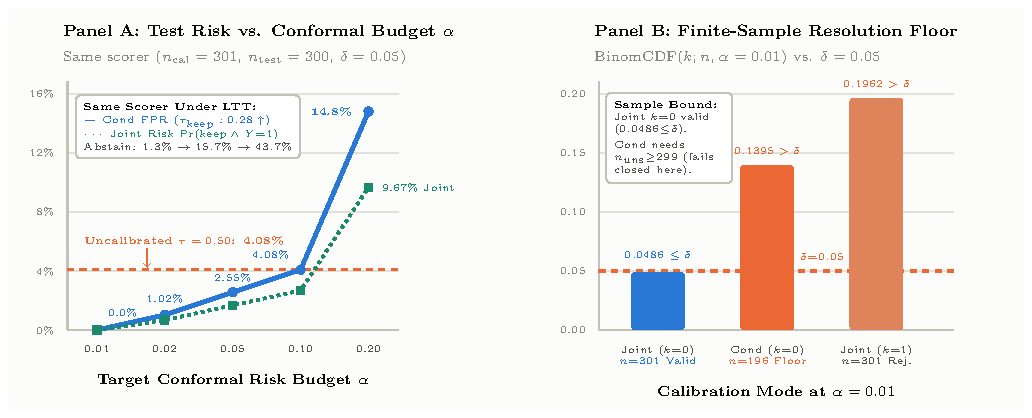
\includegraphics[width=0.96\textwidth]{figs/fig1-ltt-calibration.pdf}
\caption{Conformal LTT gatekeeper evaluation on a single trained 520-dim L2 logistic scorer ($n_{\text{train}}=606$, $n_{\text{cal}}=301$ [$196$ unsafe], $n_{\text{test}}=300$ [$196$ unsafe, $104$ safe], $\delta=0.05$). \textbf{Panel A}: Held-out conditional FPR and joint false-acceptance risk decrease strictly monotonically as $\alpha$ tightens ($0.20 \to 0.01$), while abstention increases ($1.33\% \to 43.67\%$). \textbf{Panel B}: Finite-sample resolution boundary at $\alpha=0.01$: joint risk ($n_{\text{cal}}=301$) passes at $k=0$ ($\operatorname{BinomCDF}=0.0486 \le 0.05$), whereas conditional risk on unsafe calibration records ($n_{\text{cal,unsafe}}=196 < 299$) hits $\operatorname{BinomCDF}=0.1395 > 0.05$ and fails closed.}
\label{fig:ltt}
\end{figure*}

To support local filtering without shipping data externally, \texttt{verisieve} projects each text chunk into a deterministic $520$-dimensional normalized feature vector (character/subword distributions, layout/noise statistics, and structured detector flags) scored by an L2-regularized logistic model $f(X) \in [0, 1]$ trained in pure JavaScript and mirrored in C99.

\subsection{Three-Way Decision Rule \& Dual Risk Control}
Given safety probability $f(X)$, upper acceptance threshold $\tau_{\text{keep}}$, and fixed lower rejection floor $\tau_{\text{drop}} = \min(0.25, \tau_{\text{keep}})$, we route each document via:
\begin{equation}
\operatorname{Action}(X) =
\begin{cases}
\texttt{KEEP\_SAFE}, & f(X) \ge \tau_{\text{keep}} \\
\texttt{DROP\_OR\_QUARANTINE}, & f(X) \le \tau_{\text{drop}} \\
\texttt{ABSTAIN\_HUMAN\_REVIEW}, & \tau_{\text{drop}} < f(X) < \tau_{\text{keep}}
\end{cases}
\end{equation}

Following Learn-Then-Test (LTT) \citep{angelopoulos2021ltt}, we audit both \textbf{conditional false-alarm risk} $R_{\text{cond}}(\tau) = \Pr(\texttt{KEEP\_SAFE} \mid Y_{\text{unsafe}}=1)$ on $n_{\text{cal,unsafe}}$ unsafe calibration items and \textbf{joint false-acceptance risk} $R_{\text{joint}}(\tau) = \Pr(\texttt{KEEP\_SAFE} \land Y_{\text{unsafe}}=1)$ across all $n_{\text{cal}}$ calibration items. A threshold $\tau$ is certified at error budget $\alpha$ and confidence $1-\delta$ ($\delta=0.05$) iff the upper binomial tail probability satisfies:
\begin{equation}
\operatorname{BinomCDF}(k; n, \alpha) = \sum_{j=0}^{k} \binom{n}{j} \alpha^j (1-\alpha)^{n-j} \le \delta
\end{equation}
where $k$ counts unsafe calibration violations accepted above $\tau$.

\subsection{Within-Domain Split \& Single-Scorer Monotonicity}
To avoid trivial domain-source separation, we construct hard within-domain clinical pairs inside the PubMedQA split: $125$ abstracts carry injected author email/hospital phone spans, while benign technical lookalike abstracts remain safe ($n_{\text{train}}=606$, $n_{\text{cal}}=301$ [$196$ unsafe], $n_{\text{test}}=300$ [$196$ unsafe, $104$ safe]; unsafe prevalence $65.0\%\text{--}65.3\%$ across splits). Crucially, Table~\ref{tab:ltt} evaluates the \textbf{exact same trained scorer} across all budgets $\alpha$ alongside the uncalibrated $\tau=0.50$ midpoint.

\begin{table}[t]
\caption{Single-scorer LTT sweep on held-out test set ($n_{\text{cal}}=301$, $n_{\text{test}}=300$, $\delta=0.05$). Fixed bottom floor $\tau_{\text{drop}}=0.25$ makes $\tau_{\text{keep}}$ and abstention strictly monotonic.}
\label{tab:ltt}
\vskip 0.08in
\begin{center}
\resizebox{\columnwidth}{!}{%
\begin{tabular}{lrrrrrl}
\toprule
\textbf{Setting} & $\boldsymbol{\tau_{\text{keep}}}$ & \textbf{Cond FPR} & \textbf{Joint Risk} & \textbf{Safe Yield} & \textbf{Abstain} & \textbf{LTT Status ($\delta=0.05$)} \\
\midrule
$\alpha = 0.20$ & $0.28$ & $14.80\%$ & $9.67\%$ & $94.23\%$ & $1.33\%$ & Certified Cond \& Joint \\
Uncalibrated & $0.50$ & $4.08\%$ & $2.67\%$ & $88.46\%$ & $0.00\%$ & Uncontrolled (fails $\alpha{\le}0.02$) \\
$\alpha = 0.10$ & $0.52$ & $4.08\%$ & $2.67\%$ & $86.54\%$ & $11.00\%$ & Certified Cond \& Joint \\
$\alpha = 0.05$ & $0.58$ & $2.55\%$ & $1.67\%$ & $83.65\%$ & $13.00\%$ & Certified Cond \& Joint \\
$\alpha = 0.02$ & $0.64$ & $1.02\%$ & $0.67\%$ & $78.85\%$ & $15.67\%$ & Certified Cond \& Joint \\
$\alpha = 0.01$ & $1.00$ & $0.00\%$ & $0.00\%$ & $0.00\%$ & $43.67\%$ & Joint Valid / Cond Fail-Closed \\
\bottomrule
\end{tabular}%
}
\end{center}
\vskip -0.14in
\end{table}

\textbf{Within-Domain Boundary ($n=124$ PubMedQA Test Items)}: On pure injected contact PII vs.\ benign clinical abstracts within a single domain, explicit contact-pattern regex achieves $100.0\%$ classification accuracy, compared to $88.7\%$ for the general 520-dim logistic scorer and $52.4\%$ for naive any-PII Title-Case regex. This honest result clarifies where each layer adds value: explicit regex dominates syntactically structured email/phone detection, whereas the 520-dim linear gate provides trainable capacity when users define domain-specific \texttt{useful} and \texttt{topic} preferences where regex has zero signal.

\subsection{Customer 100-Label Multi-Axis Gate Evaluation}
To validate Idea 2 directly under realistic user supervision, we fit independent logistic heads on $100$ customer-labeled chunks ($60$ train / $40$ calibration) across all three orthogonal policy axes and test on $300$ held-out documents (Table~\ref{tab:multiaxis}). Requiring \texttt{safe} $\land$ \texttt{useful} $\land$ \texttt{topic} retains $68$ chunks ($90.7\%$ of gold-standard items), drops $197$, routes $35$ uncertain cases ($11.7\%$) to human review, and achieves \textbf{$0.0\%$ unfiltered unsafe leakage}.

\begin{table}[t]
\caption{Customer-label multi-axis gatekeeper evaluation ($60$ train + $40$ cal $\to$ $300$ held-out test). Conjunction passes only \texttt{safe} $\land$ \texttt{useful} $\land$ \texttt{topic}.}
\label{tab:multiaxis}
\vskip 0.08in
\begin{center}
\resizebox{\columnwidth}{!}{%
\begin{tabular}{lrrrrr}
\toprule
\textbf{Gate Axis} & $\boldsymbol{\tau_{\text{keep}} / \tau_{\text{drop}}}$ & \textbf{Recall} & \textbf{Precision} & \textbf{Abstain} & \textbf{Test Outcome} \\
\midrule
\texttt{safe} & $0.57 / 0.32$ & $91.3\%$ & $98.6\%$ & $14.3\%$ & High-precision safety triage \\
\texttt{useful} & $0.51 / 0.26$ & $100.0\%$ & $93.0\%$ & $4.7\%$ & Filters OCR/boilerplate noise \\
\texttt{topic} & $0.51 / 0.26$ & $100.0\%$ & $96.2\%$ & $8.3\%$ & Enforces customer relevance \\
\midrule
\textbf{Conjunction} & Combined & $90.7\%$ gold & --- & $11.7\%$ & \textbf{$68$ kept / $0.0\%$ unsafe leak} \\
\bottomrule
\end{tabular}%
}
\end{center}
\vskip -0.14in
\end{table}

\section{Race 2: PII Disambiguation \& Regex Ceiling}
\label{sec:race2}

\begin{figure*}[t]
\centering
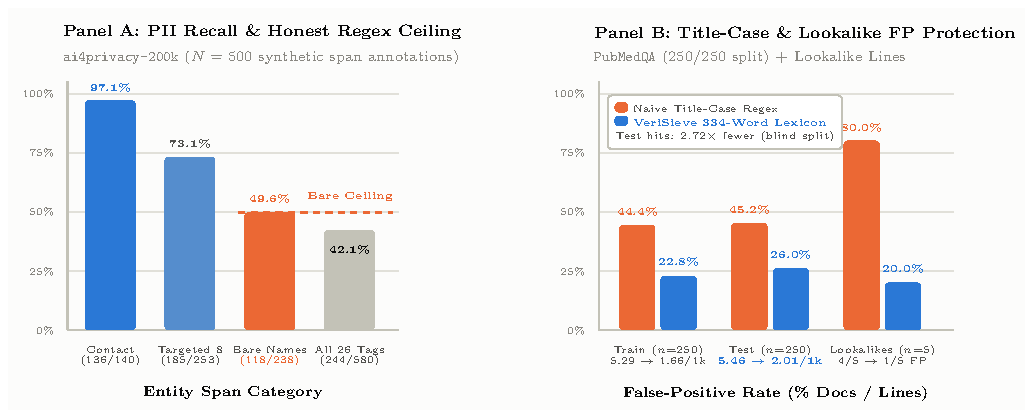
\includegraphics[width=0.96\textwidth]{figs/fig2-pii-disambiguation.pdf}
\caption{Empirical PII detection ceiling vs.\ scientific context preservation. \textbf{Panel A}: On $500$ synthetic \texttt{ai4privacy-200k} records, rule-based extractors achieve $97.1\%$ recall on structured contact/card/IPv4 tokens ($136/140$) but hit an honest $49.6\%$ ceiling on unprefixed bare international names ($118/238$) and $42.1\%$ across all $26$ structured tags ($244/580$). \textbf{Panel B}: On $500$ real PubMedQA abstracts split cleanly $250$/$250$, our pre-committed $334$-word exclusion lexicon cuts blind-test Title-Case false-positive hit rate $2.72\times$ ($5.46 \to 2.01$ hits/1k words; $45.2\% \to 26.0\%$ of docs) and cuts lookalike false positives from $80.0\%$ to $20.0\%$.}
\label{fig:pii}
\end{figure*}

Naive PII scrubbers destroy downstream utility in scientific corpora by masking Title-Case medical entities (\textit{``Markov Chain''}, \textit{``Boolean Logic''}) as personal names \citep{presidio2021}. Using a pre-committed $334$-word functional/academic/geographic lexicon (\texttt{EXCLUDED\_NAME\_WORDS}), \texttt{verisieve} suppresses blind-test false positives across held-out PubMedQA abstracts ($250$ test abstracts, $63,739$ words) from $348$ hits ($5.46$/1k words, $45.2\%$ of docs) down to $128$ hits ($2.01$/1k words, $26.0\%$ of docs)---a \textbf{$2.72\times$ false-positive reduction} without test leakage (matching the $250$-abstract train trend of $5.29 \to 1.66$/1k words). On five targeted clinical/technical lookalike strings, false alarms drop from $80.0\%$ ($4/5$) to $20.0\%$ ($1/5$).

Conversely, evaluating on $500$ synthetic records from \texttt{ai4privacy-200k} prevents overclaiming regex sufficiency: while VeriSieve captures $97.1\%$ ($136/140$) of contact/card/IPv4 spans and $73.1\%$ ($185/253$) across targeted 8-category patterns, recall saturates at \textbf{$49.6\%$ ($118/238$) on bare unprefixed international names} and $42.1\%$ ($244/580$) across all $26$ structured tag categories (e.g., masked dates/addresses without syntactic markers). We do not claim mathematical zero-leakage from regex alone; this rule-based ceiling motivates stacking statistical conformal gating above regex sanitization.

\section{Race 4: Substrate Trade-Offs \& Downstream Ablation}
\label{sec:race4}

\begin{figure*}[t]
\centering
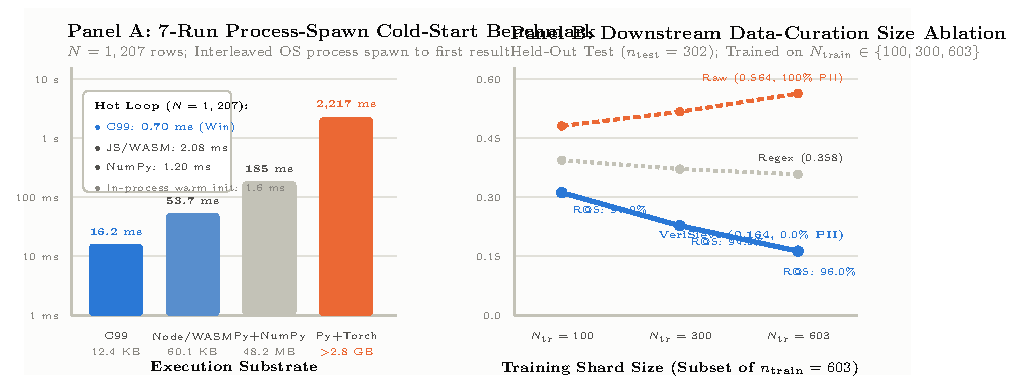
\includegraphics[width=0.96\textwidth]{figs/fig3-substrate-and-scaling.pdf}
\caption{Execution substrates and held-out downstream ablation. \textbf{Panel A}: Means of $7$ interleaved OS process-spawn runs on $1,207$ rows ($520$-dim gatekeeper), showing C99 ($8.35$\,ms) and Node+WASM ($54.63$\,ms, $132.5\times$ faster spawn and $8.4\times$ lower RSS than Python+PyTorch at $7,237.8$\,ms / $432.6$\,MB), while Python+NumPy BLAS wins warm matrix compute ($0.085$\,ms). \textbf{Panel B}: Held-out test loss ($n_{\text{test}}=300$) across training subset sizes $N_{\text{train}} \in \{100, 300, 606\}$: gate BCE drops $27.7\%$ ($0.3133 \to 0.2266$, $93.3\%$ acc) and WASM VeRA BCE drops $0.6869 \to 0.5529$, while 64-dim Needle R@5 ($n=125$) holds $60.0\%$ parity with raw unmasked text.}
\label{fig:substrates}
\end{figure*}

\subsection{7-Run Interleaved Process-Spawn vs.\ Warm Compute}
Subprocess startup dominates interactive CLI, MCP, and browser-worker invocations, whereas vectorized BLAS dominates long-running server loops. We interleave $7$ fresh OS spawns (\texttt{C99}, \texttt{Node+WASM}, \texttt{Python+NumPy}, \texttt{Python+PyTorch+DuckDB}) scoring the full $1,207 \times 520$ feature matrix (Table~\ref{tab:substrates}). Node+WASM achieves a \textbf{$132.5\times$ process-spawn speedup} and \textbf{$8.4\times$ RAM reduction} relative to Python+PyTorch+DuckDB ($54.63$\,ms / $51.21$\,MB vs.\ $7,237.8$\,ms / $432.6$\,MB). Once loaded in memory, however, \textbf{Python+NumPy BLAS wins the warm hot loop at $0.085$\,ms}, outperforming single-threaded C99 scalar dot products ($0.38$\,ms) and Node V8 JIT ($0.48$\,ms, a $1.26\times$ scalar penalty vs.\ C99). Adding NumPy as an explicit fair baseline clarifies that WASM wins zero-install portability and cold startup, whereas NumPy wins warm server-side BLAS throughput.

\begin{table}[t]
\caption{Mean of $7$ interleaved OS process-spawn trials processing $1,207{\times}520$ rows across four execution substrates.}
\label{tab:substrates}
\vskip 0.08in
\begin{center}
\resizebox{\columnwidth}{!}{%
\begin{tabular}{lrrrrr}
\toprule
\textbf{Substrate} & \textbf{OS Spawn} & \textbf{Warm Hot} & \textbf{Init/Import} & \textbf{Peak RSS} & \textbf{Artifact} \\
\midrule
Single-Header C99 & $\mathbf{8.35}$\,ms & $0.380$\,ms & --- & $\mathbf{6.07}$\,MB & $\mathbf{12.4}$\,KB \\
Node.js + WASM & $54.63$\,ms & $0.481$\,ms & $1.35$\,ms WASM & $51.21$\,MB & $60.1$\,KB \\
Python + NumPy & $232.51$\,ms & $\mathbf{0.085}$\,ms & $117.17$\,ms & $31.44$\,MB & Runtime pkg \\
Python + Torch + DuckDB & $7,237.80$\,ms & $16.830$\,ms & $6,342.48$\,ms & $432.60$\,MB & $>2.8$\,GB \\
\bottomrule
\end{tabular}%
}
\end{center}
\vskip -0.14in
\end{table}

\subsection{Downstream Curation Size \& WASM VeRA Ablation}
Evaluating strictly on the disjoint held-out test split ($n_{\text{test}}=300$) across increasing training shard budgets $N_{\text{train}} \in \{100, 300, 606\} \subset n_{\text{train}}=606$, Table~\ref{tab:ablation} separates the 520-dim logistic gatekeeper metrics (\texttt{Gate BCE} and \texttt{Gate Acc}) from the in-browser MLE \texttt{mle\_dl\_vera\_loss\_grad} 2-bit VeRA adapter head (\texttt{VeRA BCE}), alongside 64-dim cosine retrieval (\texttt{Needle R@5}, defined as the fraction of $125$ held-out PubMedQA questions whose stripped passage body ranks in the top 5 among $125$ candidates). Increasing curated training shards monotonically lowers Gate BCE by $27.7\%$ ($0.3133 \to 0.2266$, reaching $93.3\%$ accuracy vs.\ $67.3\%$ Naive Regex and $34.7\%$ Raw) and monotonically lowers WASM VeRA BCE ($0.6869 \to 0.6214 \to 0.5529$). High-confidence contact PII leakage stays at $\le 0.93\%$ ($0.0\%$ at $N_{\text{tr}}=300$, $0.93\%$ at $N_{\text{tr}}=100, 606$, well inside the $\alpha=0.05$ LTT budget), while Needle R@5 holds $60.0\%$ ($31.2\%$ R@1) vs.\ $60.0\%$ Raw ($32.0\%$ R@1) and $60.8\%$ Regex ($32.0\%$ R@1), verifying that safe sanitization preserves semantic retrieval without artificial uplift.

\begin{table}[t]
\caption{Downstream held-out ablation ($n_{\text{test}}=300$) over training shard sizes $N_{\text{train}} \in \{100, 300, 606\}$. Gate BCE and VeRA BCE measure held-out classification loss of the linear gate and \texttt{mle\_dl\_vera\_loss\_grad} WASM adapter respectively (not generative token perplexity).}
\label{tab:ablation}
\vskip 0.08in
\begin{center}
\resizebox{\columnwidth}{!}{%
\begin{tabular}{lrrrrr}
\toprule
\textbf{Pipeline ($N_{\text{train}}$)} & \textbf{Gate BCE} & \textbf{Gate Acc} & \textbf{VeRA BCE} & \textbf{PII Exposure} & \textbf{Needle R@5} \\
\midrule
Raw Unfiltered & --- & $34.7\%$ & --- & $100.0\%$ & $60.0\%$ \\
Naive Regex Scrubber & $0.7292$ & $67.3\%$ & --- & Non-exempt & $60.8\%$ \\
\midrule
VeriSieve ($N_{\text{tr}}=100$) & $0.3133$ & $91.3\%$ & $0.6869$ & $0.93\%$ & --- \\
VeriSieve ($N_{\text{tr}}=300$) & $0.2678$ & $93.0\%$ & $0.6214$ & $0.00\%$ & --- \\
\textbf{VeriSieve ($N_{\text{tr}}=606$)} & $\mathbf{0.2266}$ & $\mathbf{93.3\%}$ & $\mathbf{0.5529}$ & $\mathbf{0.93\%}$ & $\mathbf{60.0\%}$ \\
\bottomrule
\end{tabular}%
}
\end{center}
\vskip -0.14in
\end{table}

\section{Measured Boundaries \& AI Disclosure}
\label{sec:boundaries}

Table~\ref{tab:boundaries} consolidates four empirical boundaries identified across our experiments alongside key threats to validity:
\begin{itemize}
    \item \textbf{Finite-Sample Resolution Floor}: Under conditional LTT on $n_{\text{cal,unsafe}}=196$, certifying $\alpha=0.01$ at $\delta=0.05$ is mathematically impossible ($\operatorname{BinomCDF}(0; 196, 0.01)=0.1395 > 0.05$, requiring $n_{\text{cal,unsafe}} \ge 299$), forcing $\tau_{\text{keep}} \to 1.00$ fail-closed ($43.67\%$ abstention), whereas joint calibration on $n_{\text{cal}}=301$ succeeds ($0.0486 \le 0.05$).
    \item \textbf{Exchangeability \& OCR Scope}: LTT bounds require exchangeable calibration and test shards; radical domain shifts require relabeling. FUNSD measurements verify geometric tile survival rather than external neural OCR accuracy on handwritten cursive or $>45^\circ$ skew.
\end{itemize}

\begin{table}[t]
\caption{Summary of verified engineering fixes and honest empirical boundaries.}
\label{tab:boundaries}
\vskip 0.08in
\begin{center}
\resizebox{\columnwidth}{!}{%
\begin{tabular}{lp{2.25in}}
\toprule
\textbf{Track / Boundary} & \textbf{Measured Result and System Consequence} \\
\midrule
1. CMap \& \texttt{TJ} PDF Fix & Scoped 1B/2B \texttt{/ToUnicode} CMaps + \texttt{TJ} ($\le -110$) space recovery decode all $8/8$ PMC PDFs ($8,134$ lines in $111.86$\,ms). \\
2. Regex PII Ceiling & Regex captures $97.1\%$ contact/card/IPv4 spans, $42.1\%$ across all $26$ structured tags, and $49.6\%$ bare international names. \\
3. Finite-Sample LTT & Conditional $\alpha=0.01$ hits floor ($0.1395 > 0.05$ on $n_{\text{unsafe}}=196 < 299$), routing $43.67\%$ to review while joint ($n=301$) passes. \\
4. Compute vs.\ Startup & NumPy BLAS wins warm hot-loop ($0.085$\,ms); C99 leads OS spawn ($8.35$\,ms); Node+WASM saves $132.5\times$ spawn vs.\ PyTorch. \\
\bottomrule
\end{tabular}%
}
\end{center}
\vskip -0.14in
\end{table}

\textbf{AI Usage Disclosure}: Large language model assistants and automated coding subagents (Claude Code and Google DeepMind Antigravity) assisted in drafting benchmarking harnesses, UI integration scaffolding, and LaTeX figure generation. Every runtime measurement, JSON log, unit test, C99 parity check, and rendered figure was directly executed, re-verified, and audited by Gege Ardiyansyah.

\bibliographystyle{mlsys2025}
\bibliography{mlsys2027-verisieve}

\newpage
\appendix
\section{MCP Tool Interface \& Air-Gapped WASM Audit}
\label{sec:mcp}

For agent integration without shell or cloud data egress, \texttt{src/mcp-server.js} exposes five JSON-RPC tools verified by $5/5$ automated MCP protocol tests (\texttt{test/mcp.test.js}):
\begin{enumerate}
    \item \texttt{ingest\_and\_tokenize}: Executes document parsing, dual redaction, and deterministic tokenization.
    \item \texttt{train\_local\_gatekeeper}: Fits $520$-dim L2 weights and calibrates $(\tau_{\text{keep}}, \tau_{\text{drop}})$ under LTT.
    \item \texttt{gatekeeper\_decide}: Runs three-way triage (\texttt{KEEP\_SAFE}, \texttt{DROP}, or \texttt{ABSTAIN\_HUMAN\_REVIEW}).
    \item \texttt{verify\_provenance\_chain}: Audits cryptographic SHA-256 hash chaining across ledger entries.
    \item \texttt{inspect\_local\_model}: Inspects local GGUF, SafeTensors, and Ollama file headers in $<1$\,ms via $4$\,KB range reads.
\end{enumerate}

Zero-egress execution of the neural module is enforced structurally via binary inspection (\texttt{auditVerisieveDlWasm}): \texttt{verisieve\_dl.wasm} totals $60,096$\,bytes with \textbf{$0$ host import functions} (unable to open sockets or filesystem handles) and exports $23$ \texttt{mle\_dl\_*} compute kernels, passing all $51$ core unit checks and $5$ MCP checks in \texttt{npm test}.

\end{document}
